\documentclass[cjk,c,squeeze,shrink,dvipdfmx,12pt]{beamer}
% 以下は決まり文句
\usepackage{bxdpx-beamer}                      % dvipdfmx用の fix
\usepackage{pxjahyper}                         % 日本語で'しおり'
\usepackage{minijs}                            % min10ヤダ
\usepackage{pgfgantt} % For release_cycle.tex
\usepackage{chronology}
\usepackage{color}
\renewcommand{\kanjifamilydefault}{\gtdefault} % 既定をゴシック体に

\usetheme{KansaiDebian}
\usepackage{amsmath,amssymb,ulem}
\AtBeginSection[]{%
  \begin{frame}<beamer>\frametitle{Agenda}\tableofcontents[currentsection]\end{frame}}

\title[Debian Updates: Buster]{Debian Updates: Buster}
\subtitle[KOF 2019]{関西オープンフォーラム 2019}
\author[おおつき]{Yosuke OTSUKI}
  
\institute[Debian JP Project]{%
  {\footnotesize{%
      Debian JP Project/関西Debian勉強会
    }}
}
\date[2019/08/03]{%
  {\tiny{2019年11月09日@ 大阪南港 ATC}}
}

\begin{document}
\setbeamercovered{transparent}
\takahashi[80]{ }
{%
  \setbeamertemplate{headline}{}
  \setbeamertemplate{footline}{}
  \begin{frame}
    \maketitle
  \end{frame}
}

\begin{frame}[fragile]
  \frametitle{Disclaimer}
  \begin{itemize}
  \item 疑問、質問、ツッコミ、茶々、\alert{大歓迎}
  \item その場でインタラクティブにどうぞ
  \item ハッシュタグ \alert{\#debianjp} で
  \end{itemize}
\end{frame}

\begin{frame}[fragile]{Agenda}
  \tableofcontents
\end{frame}
%-------------------


\section{Debianとは? Debian JP とは?}
\takahashi[60]{Debianとは?}


\begin{frame}[fragile]{Debian とは?}

  \alert{フリー/オープン}な\alert{ユニバーサル}オペレーティングシステムを
  作成しようとするボランティアベースのプロジェクト。

  \vfill
  \centering
  \begin{tabular}{|c|c|c|}
    \hline
    ディストリ & 企業 & ボランティア \\ \hline
    Fedora & RedHat支援あり & あり  \\ \hline
    RHEL & RedHat & なし  \\ \hline
    CentOS & RedHat支援あり & あり \\ \hline
    \color{red}{Debian}  & \color{red}{なし} & \color{red}{あり} \\ \hline
    Ubuntu  & Canonical & あり \\ \hline
    openSUSE & SUSE支援あり & あり \\ \hline
    SLES & SUSE & なし \\ \hline
  \end{tabular}
  \vfill
\end{frame}


%-----------------------------------------------------
% Source
%-----------------------------------------------------
%Figure taken from https://clarity.desgin accessed 2019/Nov/04
%
%-----------------------------------------------------
% Clarity MIT License
%-----------------------------------------------------
%Clarity
%
%Copyright © 2016-2018 VMware, Inc.  All rights reserved
%
%The MIT license (the License) set forth below applies to all parts of the Clarity project except for the fonts which are licensed under the SIL Open Font License version 1.1.  You may not use this file except in compliance with the License.
%
%MIT License
%
%Permission is hereby granted, free of charge, to any person obtaining a copy of this software and associated documentation files (the Software), to deal in the Software without restriction, including without limitation the rights to use, copy, modify, merge, publish, distribute, sublicense, and/or sell copies of the Software, and to permit persons to whom the Software is furnished to do
%so, subject to the following conditions:
%
%The above copyright notice and this permission notice shall be included in all copies or substantial portions of the Software.
%
%THE SOFTWARE IS PROVIDED AS IS, WITHOUT WARRANTY OF ANY KIND, EXPRESS OR IMPLIED, INCLUDING BUT NOT LIMITED TO THE WARRANTIES OF MERCHANTABILITY, FITNESS FOR A PARTICULAR PURPOSE AND NONINFRINGEMENT. IN NO EVENT SHALL THE AUTHORS OR COPYRIGHT HOLDERS BE LIABLE FOR ANY CLAIM, DAMAGES OR OTHER LIABILITY, WHETHER IN AN ACTION OF CONTRACT, TORT OR OTHERWISE, ARISING FROM, OUT OF OR IN CONNECTION WITH THE SOFTWARE OR THE USE OR OTHER DEALINGS IN THE SOFTWARE.

\begin{frame}[fragile]{Debian の開発}
	\begin{center}
	\begin{tabular}{ccc}
	
\includegraphics[scale=0.2]{template-kansai/images/user-solid.eps}	
	&
		${\Huge \leftarrow}$
	&
	
\includegraphics[scale=0.2]{template-kansai/images/user-solid.eps}	
	\\
	Debian & & Upstream {\tiny(開発元: Python, gcc など)}
	\end{tabular}
	\end{center}
	%\begin{itemize}
	%\item Debian の Developer・Maintainer が Debian に移植
	%\item Debian 発祥のプロジェクトもある。例 apt など
	%\end{itemize}

	\hspace{1em}
	Taken from \url{https://clarity.desgin}, MIT License
\end{frame}



\begin{frame}[fragile]{Debian とは?}
  厳格/厳密なポリシーとガイドラインに沿った開発体制
  \begin{itemize}
  \item Debian 社会契約
  \item Debian フリーソフトウェアガイドライン
    \begin{itemize}
    \item オープンソースの定義の元
    \end{itemize}
  \item Debian Policy
  \end{itemize}
\end{frame}

\begin{frame}[fragile]{Debian とは?}
  \begin{columns}
    \begin{column}{.58\paperwidth}
      \begin{itemize}
      \item
        他のディストリビューションのベースとなっている
	\begin{itemize}
	  \item Ubuntu, Rasbian
	\end{itemize}
      \item
        Debian 派生ディストリビューションとの協力体制の整備
      \end{itemize}
    \end{column}
    \begin{column}{.4\paperwidth}
      \centering
      % https://upload.wikimedia.org/wikipedia/commons/thumb/6/69/DebianFamilyTree1210.svg/500px-DebianFamilyTree1210.svg.png
      % \includegraphics[height=.65\paperheight]{image201908/500px-DebianFamilyTree1210.png}
    \end{column}
  \end{columns}
\end{frame}

%\begin{frame}[fragile]{Debian とは?}
% 世界規模で開発が行われており、63ヶ国、約1,100名のDebian公式開発者が開発を行
% っている。パッケージメンテナや翻訳などの貢献者も入れるともっと多くの開発者が参加
% していることになる。
%
% \centering
% % https://wiki.debconf.org/upload/thumb/d/da/Dc17logo.png/800px-Dc17logo.png
% % \includegraphics[width=0.4\linewidth]{image201908/800px-Dc17logo.png}
% % https://wiki.debconf.org/upload/thumb/6/60/DebConf18_Horizontal_Logo.png/800px-DebConf18_Horizontal_Logo.png
% % \includegraphics[width=0.4\linewidth]{image201908/800px-DebConf18_Horizontal_Logo.png}
%\end{frame}


\begin{frame}[fragile]{Debian とは?}
  2019年11月の時点で、
  \pause
  \begin{itemize}[<+->]
  \item
    最新版は {\alert{Debian 10}}, Buster
  \item
    提供パッケージ数は{\alert{約59,000}}
  \item
    公式にサポートするCPUアーキテクチャは{\alert{10}}
  \item {\alert{約2年毎}}にリリース
    %\begin{itemize}
    %\item 3 年のサポート, 5 年の LTS サポート
    %\end{itemize}
  \end{itemize}
\end{frame}


%-----------------------------
% Required
%-----------------------------
%\usepackage{bchart}
%\usepackage{chronology}
%
\begin{frame}[fragile]{$B%j%j!<%9%5%$%/%k$H%5%]!<%H4|4V(B}
	\begin{bchart}[step=2, max=5]
		\bcbar[text=$B%j%j!<%9%5%$%/%k(B]{2}
			\bigskip
		\bcbar[text=$BI8=`%5%]!<%H4|4V(B]{3}
			\smallskip
		\bcbar[text=Long Term Support (LTS)]{5}
	\end{bchart}
	\begin{itemize}
		\item Debian $B$r%Y!<%9$K99$KD9$$4|4V%5%]!<%HDs6!$9$k%W%m%8%'%/%H$b$"$k(B
	\end{itemize}
\end{frame}


\begin{frame}[fragile]{Debian とは?: まとめ}
  \pause
  \begin{itemize}[<+->]
  \item ボランティアベースのプロジェクト
  \item Debianはフリー/オープンなOS
  \item 厳格なパッケージングポリシー
  \item 約2年毎にリリース
   \end{itemize}
\end{frame}

%------------------
\begin{frame}[fragile]{Debian JP Project とは?\\[-.5em]{\normalsize{\texttt{https://www.debian.or.jp}}}}
  \pause
  \begin{itemize}[<+->]
  \item 日本でのDebianの普及を目的とした任意団体。
  \item %
    Debianの日本語による情報発信、
    ユーザとの情報交換、
    Debian 開発者、
    パッケージメンテナの育成など。
  \end{itemize}
\end{frame}


\begin{frame}
  \frametitle{Debian勉強会とは?%
    \\[-.5em]{\normalsize{\texttt{https://tokyodebian-team.pages.debian.net/}}}%
    \\[-.5em]{\normalsize{\texttt{https://wiki.debian.org/KansaiDebian}}}%
  }
  \pause
  \begin{itemize}[<+->]
  \item
    2005年1月開始, Debian Developer 上川さん発起人
  \item
    東京と関西で月に一回コンスタントに開催しているDebian開発者、
    ユーザによる勉強会。
  \item
    何がしたいのか?
    \begin{itemize}[<+->]
    \item
      MLとIRCで情報交換⇒face-to-faceであう場所がない
    \item
      まとまったドキュメントが出てこない
    \end{itemize}
  \item
    Debian勉強会でやっていること
    \begin{itemize}[<+->]
    \item
      定期的に集まる(場の提供)
    \item
      資料を作成して, 公開(GPL-2+) \\
      {\small \url{https://salsa.debian.org/tokyodebian-team/}}
    \end{itemize}
  \end{itemize}

\end{frame}

\begin{frame}[fragile]{Debconf}
  \begin{itemize}
  \item 年に一回, Debian 開発者が集って開催するカンファレンス
    \begin{itemize}
      \item 2019/07/21 - 07/28: Debconf19: CURITIBA - BRAZIL
      \item 2020/08/23 - 08/29: Debconf20: Haifa - Israel
    \end{itemize}
  \end{itemize}
  \begin{center}
     % https://bits.debian.org/2019/07/debconf19-closes.html
     %\includegraphics[scale=0.2]{image201911-kansai/debconf19_group_small.jpg}
  \end{center}
\end{frame}

%-----------------------
\takahashi[40]{Any Questions?}

\section{Debian Updates: Buster}
\takahashi[60]{Debian Updates: Buster}

{%
  \setbeamertemplate{headline}{}
  \setbeamertemplate{footline}{}
  \begin{frame}
    \centering
    % https://bits.debian.org/images/upcoming-buster.png
    % \includegraphics[scale=1]{image201908/upcoming-buster.png}
  \end{frame}
}

\takahashi[60]{Debian 10 Buster Released!}


\begin{frame}[fragile]{%
    Debian Updates: Buster%
    \\[-.5em]{\normalsize{Release Timetable}}
	}
	\begin{chronology}[9]{2015}{2019}{21cm}{23cm}
		\event{\decimaldate{9}{11}{2014}}{\color{red}2014/Nov/09 時期リリースの名前が決定: Buster}
		\event{\decimaldate{26}{4}{2015}}{2015/Apr/26 Debian 8 Jessie リリース}
		\event{\decimaldate{17}{6}{2017}}{2017/June/07 Debain 9 Stretch リリース。{\color{red}Buster が Testing になる}}
		\event{\decimaldate{12}{1}{2019}}{{\tiny \color{red}2019/Jan/12 Transition Freeze}}
		\event{\decimaldate{12}{2}{2019}}{{\tiny \color{red}2019/Feb/12 Soft Freeze}}
		\event{\decimaldate{12}{3}{2019}}{{\tiny \color{red}2019/Mar/12 Full Freeze}}
		\event{\decimaldate{6}{7}{2019}}{{\color{red}2019/Jul/06 Debian 10 Buster リリース}}
		\event{\decimaldate{7}{9}{2019}}{{\color{red}2019/Sep/07 10.1 リリース}}
		\event{\decimaldate{16}{11}{2019}}{{\color{red}2019/Nov/16 10.2 リリース (予定)}}
	\end{chronology}
	Bullseye はだいたい 2021 年夏ぐらい?
\end{frame}
%\begin{frame}[fragile]{%
%    Debian Updates: Buster%
%    \\[-.5em]{\normalsize{Release Timetable}}
%  }
%  \pause
%  \begin{itemize}[<+->]
%  \item 2014/11/09: Distribution codename announced
%  \item 2017/06/17: Stretch is released, and buster becomes testing
%  \item 2019/01/12: Transition freeze
%  \item 2019/02/12: Soft freeze
%  \item 2019/03/12: Full freeze
%  \item 2019/07/06: Released!
%  \item (2019/09/07: Updated Debian 10.1 released)
%  \end{itemize}
%\end{frame}

%\begin{frame}[fragile]{%
%    Debian Updates: Buster%
%    \\[-.5em]{\normalsize{Artwork}}
%  }
%  \begin{itemize}
%  \item Alex Makas: futurePrototype
%  \end{itemize}
%  \begin{center}
%    
\includegraphics[width=0.8\hsize]{image201906/futurePrototype-wallpaper-1920x1080.png}
%  \end{center}
%\end{frame}

\begin{frame}[fragile]{%
    Debian Updates: Buster%
    \\[-.5em]{\normalsize{Architectures}}
  }
  \begin{itemize}
  \item amd64, i386
  \item arm64, armel, armhf
  \item mips64el, mipsel, mips
  \item ppc64el
  \item s390x
  \end{itemize}
\end{frame}

\begin{frame}[fragile]{%
    Debian Updates: Buster%
    \\[-.5em]{\normalsize{Packages \& versions}}
  }
  \begin{itemize}
  \item GNOME 3.30, KDE Plasma 5.14, Cinnamon 3.8, MATE 1.20, Xfce 4.12, LXDE 0.99.2, LXQt 0.14
  \item Linux 4.19 series
  \item Chromium 73.0, Firefox 60.7, Thunderbird 60.7.2
  \item LibreOffice 6.1, GIMP 2.10.8, Inkscape 0.92.4
  \item GNU Compiler Collection 7.4 and 8.3, Clang-6.0.1 and 7.0.1
  \item Perl 5.28, Python 3.7.2, Ruby 2.5.1, PHP 7.3, Golang 1.11, OpenJDK 11, Rustc 1.34
  \item MariaDB 10.3, PostgreSQL 11
  \item Emacs 26.1, Vim 8.1
  \item etc..
  \end{itemize}
\end{frame}

\begin{frame}[fragile]{%
    Debian Updates: Buster%
    \\[-.5em]{\normalsize{New Features (1)}}
  }
  UEFI セキュアブート

  \begin{itemize}
  \item セキュアブートが有効な状態でもインストールと利用ができるようになった
  \item shim-signed, grub-efi-\{amd64,ia32\}-signed, Buster の Linux カーネルパッケージをインストールすれば既存の Debian でも利用可能
  \item DKMS が使用できないなど一部機能の制限あり
  \end{itemize}
\end{frame}

\begin{frame}[fragile]{%
    Debian Updates: Buster%
    \\[-.5em]{\normalsize{New Features (2)}}
  }

  AppArmorがデフォルトで有効化

  \begin{itemize}
  \item 多くのプロファイルは apparmor-profiles-extra をインストールすると利用可能
  \item Linux カーネルパッケージで推奨 (Recommends) 依存設定
  \end{itemize}
\end{frame}

\begin{frame}[fragile]{%
    Debian Updates: Buster%
    \\[-.5em]{\normalsize{New Features (3)}}
  }

  ネットワークフィルタリングの nftables への変更

  \begin{itemize}
  \item iptables コマンドは nftables を使用する iptables-nft がデフォルト
  \item 従来の iptables を使用するコマンドは iptables-legacy として提供
  \item 他のディストリビューションでも同様に変更\\
    e.g. Red Hat Enterprise Linux 8.0
  \end{itemize}
\end{frame}

\begin{frame}[fragile]{%
    Debian Updates: Buster%
    \\[-.5em]{\normalsize{New Features (4)}}
  }

  GNOMEのデフォルトは Wayland

  \begin{itemize}
  \item デフォルトで Wayland を使用
  \item Xorg がデフォルトでインストール
  \end{itemize}
\end{frame}

\begin{frame}[fragile]{%
    Debian Updates: Buster%
    \\[-.5em]{\normalsize{New Features (5)}}
  }

  新規インストールは /usr マージ

\begin{verbatim}
\end{verbatim}
  \begin{center}
    {\Huge{
        \texttt{/bin → /usr/bin}\\
        \texttt{/sbin → /usr/sbin}\\
        \texttt{/lib → /usr/lib}\\
    }}
  \end{center}

  \begin{itemize}
  \item Debian 以外から提供されるソフトウェアを利用している場合は要注意
  \end{itemize}
\end{frame}

\begin{frame}[fragile]{%
    Debian Updates: Buster%
    \\[-.5em]{\normalsize{New Features (6)}}
  }
  \pause
  \begin{itemize}[<+->]
  \item APTへのセキュリティ強化オプションの追加
  \item stable ポイントリリースに対する Unattended-upgrades の挙動
  \item Cryptsetup の on-disk LUKS2への変更
  \item CUPS 2.2.10 でのドライバーレス印刷機能
  \item Allwinner A64 ベースのデバイスでの基本機能サポート
  \item などなど
  \end{itemize}
\end{frame}

\begin{frame}[fragile]{%
    Debian Updates: Buster%
    \\[-.5em]{\normalsize{Issues}}
  }
  \pause
  \begin{itemize}[<+->]
  \item glibc は Linux カーネル 3.2 以上を必要
  \item Wayland で一部アプリケーションが動作しない\\
    (synaptic, fcitx, アクセシビリティ機能)
  \item phpmyadmin, Redmine, VirtualBox などのパッケージは未収録
  \item Python2.7 は非推奨
  \item More entropy
  \item OpenSSL のデフォルトが TLS 1.2 とセキュリティレベル 2
  \item ブラウザ, レンダリングエンジン, Go 関連のパッケージは制限付きのセキュリティサポート
  \end{itemize}
\end{frame}

\begin{frame}
  \begin{itemize}
  \item 既存のPostgreSQL の再インデックス化が必要 
  \item evoluaion-ews がパッケージから消えた
  \begin{itemize}
    \item evolution で Exchange, Office365, Outlook にアクセスができなくなる 
  \end{itemize}
  \end{itemize}
\end{frame}

%\begin{frame}[fragile]{%
%    Debian Updates: Stretch%
%    \\[-.5em]{\normalsize{Debian 9.x: oldstable}}
%  }
%  \pause
%  \begin{itemize}[<+->]
%  \item 2017/06/17: Debian 9.0 released
%  \item[] :
%  \item 2019/01/23: Updated Debian 9.8 released
%  \item 2019/02/16: Updated Debian 9.9 released
%  \item 2019/04/27: Updated Debian 9.10 released
%  \item[] :
%  \item \alert{2019/07/06: Becomes oldstable}
%  \item[←] oldstable のサポートはここから 1 年
%  \item (2019/09/08: Updated Debian 9.11 released)
%  \end{itemize}
%\end{frame}



%{%
%  \setbeamertemplate{headline}{}
%  \setbeamertemplate{footline}{}
%  \begin{frame}
%    \centering
%    % https://salsa.debian.org/debconf-team/public/share/debconf19/raw/master/photos/aigarius/group/debconf19_group_small.jpg
%    % \includegraphics[width=.9\paperwidth]{image201908/debconf19_group_small.jpg}
%  \end{frame}
%}
%
%\begin{frame}[fragile]{Debian Updates: Debconf}
%  \begin{itemize}
%  \item 来年は 2020/08/23 - 08/29: Debconf20: Haifa - Israel
%    \begin{center}
%      % https://wiki.debian.org/DebConf/20/Artwork/LogoProposals?action=AttachFile&do=get&target=dc20-logo-bee.svg
%      % \includegraphics[width=.9\paperwidth]{image201908/dc20-logo-bee.png}
%    \end{center}
%  \end{itemize}
%\end{frame}


\takahashi[70]{そんな\\こんなで}

\takahashi[40]{Any Questions?}

\section{日本語によるDebianの情報}
\takahashi[40]{日本語によるDebianの情報}

\begin{frame}[fragile]{日本語によるDebianの情報}
  \begin{itemize}
  \item Debian JP Project \\
    \url{https://www.debian.or.jp}
  \item 東京エリアDebian勉強会\\
    \url{https://tokyodebian.alioth.debian.org}
  \item 関西エリアDebian勉強会 \\
    \url{https://wiki.debian.org/KansaiDebianMeeting}
  \item Twitter \\
    \url{@debian_jp}
  \item slack
    \url{debian-jp.slack.com}
  \end{itemize}
\end{frame}

\begin{frame}
  \frametitle{書籍情報}
  \begin{columns}
    \begin{column}{.5\paperwidth}
      \centering
      % http://image.gihyo.co.jp/assets/images/cover/2019/641908.jpg
      % \includegraphics[height=.6\paperheight]{image201908/sd201908.jpg}
    \end{column}
    \begin{column}{.5\paperwidth}
      \begin{itemize}
      \item %
        日本語での唯一の連載記事 \\
        「Debian Hot Topics」
      \end{itemize}
    \end{column}
  \end{columns}
\end{frame}

\begin{frame}
  \frametitle{書籍情報}
  \begin{columns}
    \begin{column}{.45\paperwidth}
      \centering
      % http://static.lulu.com/browse/product_thumbnail.php?productId=22625767&resolution=320
      % \includegraphics[height=.6\paperheight]{image201908/DebianHandbook.jpg}
    \end{column}
    \begin{column}{.54\paperwidth}
      \begin{itemize}
      \item %
        英語書籍の翻訳版
        \begin{itemize}
        \item %
          原版: The Debian Administrator's Handbook
          \begin{itemize}
          \item %
            Rapha\"el Hertzog, Roland Mas
          \item \url{https://debian-handbook.info/}
          \end{itemize}
        \end{itemize}
      \item %
        日本語で読める(現状)唯一の書籍!
      \item %
        パッケージ版:
        \texttt{debian-handbook}
      \end{itemize}
    \end{column}
  \end{columns}
\end{frame}

\takahashi[70]{そんな\\こんなで}

\begin{frame}
  \frametitle{今後のイベント}
  \begin{itemize}
  \item オープンソースカンファレンス 2019 Tokyo/Fall
    \begin{itemize}
    \item \url{https://www.ospn.jp/osc2019-fall/}
      \begin{itemize}
	\item ブース展示 11/23 日 (土) のみ
        \item 講演 11/23 日 16:15 - 17:00 3F 301 にて「Debian Updates」
      \end{itemize}
    \end{itemize}
  \item 11/24(日) 第152関西Debian勉強会
    \begin{itemize}
    \item \url{https://debianjp.connpass.com/event/155116/}
    \end{itemize}
  \end{itemize}
\end{frame}

\takahashi[40]{Any Questions?}
\takahashi[60]{Thanks!}


\begin{frame}{Clarity MIT License}
\begin{tiny}
Clarity

Copyright © 2016-2018 VMware, Inc.  All rights reserved

The MIT license (the License) set forth below applies to all parts of the Clarity project except for the fonts which are licensed under the SIL Open Font License version 1.1.  You may not use this file except in compliance with the License.

MIT License

Permission is hereby granted, free of charge, to any person obtaining a copy of this software and associated documentation files (the Software), to deal in the Software without restriction, including without limitation the rights to use, copy, modify, merge, publish, distribute, sublicense, and/or sell copies of the Software, and to permit persons to whom the Software is furnished to do
so, subject to the following conditions:

The above copyright notice and this permission notice shall be included in all copies or substantial portions of the Software.

THE SOFTWARE IS PROVIDED AS IS, WITHOUT WARRANTY OF ANY KIND, EXPRESS OR IMPLIED, INCLUDING BUT NOT LIMITED TO THE WARRANTIES OF MERCHANTABILITY, FITNESS FOR A PARTICULAR PURPOSE AND NONINFRINGEMENT. IN NO EVENT SHALL THE AUTHORS OR COPYRIGHT HOLDERS BE LIABLE FOR ANY CLAIM, DAMAGES OR OTHER LIABILITY, WHETHER IN AN ACTION OF CONTRACT, TORT OR OTHERWISE, ARISING FROM, OUT OF OR IN CONNECTION WITH THE SOFTWARE OR THE USE OR OTHER DEALINGS IN THE SOFTWARE.
\end{tiny}
\end{frame}




\end{document}
